\documentclass{article}
\usepackage[utf8]{inputenc}

\title{GU-Makro-Formler}
\author{orts }
\date{April 2016}

\usepackage{natbib}
\usepackage{graphicx}

\begin{document}

\maketitle

\section{Introduction}
Formler för makroteori. Går igenom och förklarar alla relevanta formler. 



\section{Conclusion}
``I always thought something was fundamentally wrong with the universe'' \citep{adams1995hitchhiker}

\section{Långa sikten F2-F11}
\title{Föreläsning 1}

Under krisen 2008 så sjönk BNP per capita kraftigt. Idag har den återhämtat sig så att den är på samma nivå som 2007. 

$$
    \Delta \ ln \ Z = \Delta \ln  X + \Delta \ ln Y - \Delta \ ln Q
$$
Förenkling vid förändring. Gäller vid följande. 
$$
Z = \frac{X*Y}{Q}
$$

Idag har Sverige överskott i bytesbalansen. 

Det existerar tre sätt att bestäma värdet som produceras inom ett lands gränser. 

\begin{enumerate}
    \item Användning. Summa utgifter för nya varor/tjänster för slutgiltig användnign minus import. 
    \item Produktion: summa förädlingsvärde.
    \item Inkomst: summa kaptial- och arbetsinkomster. 
\end{enumerate}

\begin{equation}
    BNP = \ Y\ = \ C + I + C^G + I^G + X - IM 
\end{equation}

Bruttonationalinkomsten, BNI: 

$$
BNI = Y + Y^F \ (Y^F: landets \ faktorinkomster.) 
$$
Faktorinkomster: ersättning till arbete och kapitel som "ägs" av landets medborgare. Det vill säga avkastning från utlandet. 

Dissponibel buruttonationalinkomst, DBNI: 

$$
DBNI = Y + Y^F + Tr^F 
$$


\textbf{Bytesbalansen}: Denna summerar flödet mellan oss och omvärlen. 

$$
Bytesbalansen = NX + Y^F + Tr^F
$$
Har vi överskott i vår bytesbalans så kan detta investeras, dvs lånas ut till andra länder. Om detta är negativt så måste vi låna från de länder som har överskott. 


Nominell BNP = löpande priser.
Real BNP = satt mot ett basår. 
\par \noindent
Tillväxttakt är $g_{t+1}$

\vspace{5mm}


\title{Föreläsning 2}
\vspace{5mm}\par

Sveriges tillväxt startade i mitten på 1800-talet. 

\textbf{Kort sikt < 2år}: Löner och priser är fasta. 

\textbf{Lång sikt 4-5år}: Löner och priser anpassar sig till jämviktsvärden. 

På kort sikt så är konjukturläget det intressanta: inflation, ränta, arbetslöshet, stabeliseringspolitik och budgettunderskott. 

\begin{enumerate}
 \item MPK = kaptialets marginalprodukt. 
 \item MPL = arbetets marginalprodukt. 
\end{enumerate}

\textbf{Prdoutktionsfunktionens egenskaper:}
\begin{enumerate}
 \item Marginalprodukterna är positiva
 \item Marginalprodukterna är avtagande
 \item Konstant skalavkastning
\end{enumerate}

Produktionsfunktion: $$ Y = F(K,N) $$
$$ Y = K^{\alpha}N^{1-\alpha}$$

E = teknisk nivå. 

$$ Y = F(K,EN)$$

\textbf{Jämviktssysselsättning (natrulig)}:
$$N^n = (1-u^n)L $$

L = arbetskraft. 

\begin{itemize}
    \item Långsiktig tillväxt är viktigare än konjukturläget för genomsnittlig inkomst.
    \item Produktionsfunktionen visar producerad kvantitet för given teknisk nivå, kaptialstock, och antal arbetare. 
\end{itemize}

\par
 
 \vspace{5mm}
 \title{Föreläsning 3}
 \vspace{5mm}
 
\par \noindent
Köpkraft = $\frac{W}{P}$, nominell lön delat med prisnivån.
Inverterad efterfrågefunktion: $P_i = P(Y_i,P,Y)$ \par \noindent

Priselasticitet: $\frac{P_i*dY_i}{dP_i*Y_i}$

Det genomsnittliga priset: 
$$
P = (1-\mu)MC = (1-\mu)\frac{W}{MPL}
$$

\textbf{Sluten ekonomi: Inkomst = produktion}
Det är köpkraften hos befolkningen som är det viktiga. Detta medför följande: 

$$
 \frac{W}{P} = \frac{MPL}{1+\mu}
$$
Om konkurrensen mellan företag ökar så minskar $ \mu$. \par \noindent

\textbf{Löneandel}: Denna är total lönesumma / nominell BNP 

$$
\frac{WN}{PY} = \frac{1-\alpha}{1+\mu}
$$

På lång sikt så når kapital per arbetare $ \frac{K}{EN} = k $ ett stabilt läge, steady state. 

\textbf{Komihåg till tenta att förklara alla modeller och formler!}

Löneandelen har legat relativt konstant under flera decennier. På ca 1/3. 
Lönesprdningen har ökat, detta kan knytas till automatiseringen. 

\vspace{5mm}
\title{Föreläsning 4} \par \noindent
\vspace{5mm}

$i_t$ är den nominella räntan mellan två perioder. Inflation är hur mycket priset förändras. Det vill säga förändringen i pris från en period till en annan. 
\textbf{Inflation: }
$$
\pi_{t+1} = \frac{P_{t+1}-P_t}{P_t}
$$

Relaränta är ungefär: $r_{t+1} \approx i_t - \pi_{t+1}$

Netto investering: 
$$
K_{t+1} - K_t = I_t -\delta K_t 
$$

\textbf{Optimala kaptialstcken: }
$$
\frac{MPK_{t+1}}{1+\mu}-\delta = r_{t+1}
$$
Ovanstående ekvation säger oss att; Det vi tjänar på att utöka kaptialstocken minus förtäringen på kapitalstocken måste vara lika med priset vi förväntas att betala för det. 


\textbf{Investeringsfunktion:} $I = I(Y^e,K,r)$

\vspace{5mm}
\title{Föreläsning 5}
\vspace{5mm}
\par \noindent

\textbf{Konsumption:} Denna bestäms av inkomsten idag, konsumtionen idag och inkomst i nästa period. 

$$
C_2 = Y^l_2 + (1+r)(Y^l_1-C_1)
$$

$$
\frac{U'(C1_)}{U'(C_2)} = \frac{1+r}{1+\rho}
$$
Den subjektiva räntan $ \rho $ bestämmer hur vida personen annser att det är mer värdefullt att spendera pengar i denna perioden jämfört med nästa. 

\textbf{Konsumptionfunktion:} $ C = C(Y,Y^e,r,A)$

Om den reala räntan ökar så vill befolkningen öka sitt sparande också, då du får mer för dina sparade pengar. Med ökad ränta så sjunker konsumtion och investeringar. 

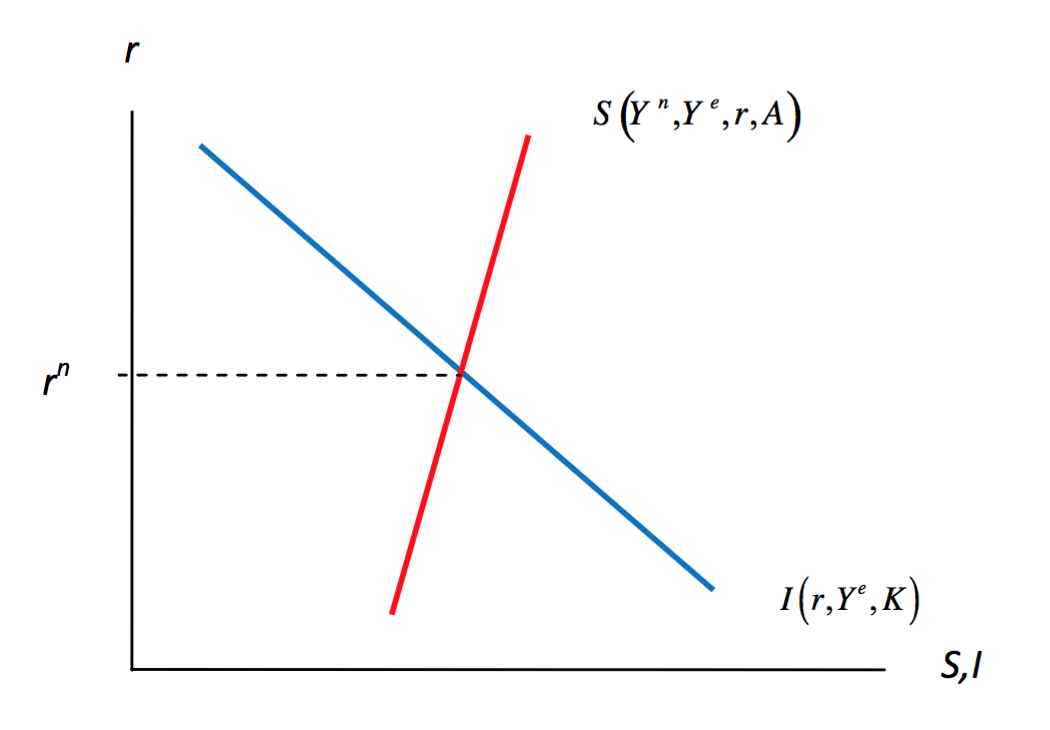
\includegraphics[scale=0.4]{skarm2}

\vspace{5mm}
\title{Föreläsning 7}
\vspace{5mm}
\par \noindent

Den optimala kapitalstocken är också villkor för den långsiktiga jämviktsnivån. 
Genom att ta fram Kaptialets marginalprodukt och sätta in så får vi ut $K^*$.  Detta på lång sikt. På kort sikt kan vi endast kolla på hur det förändrar $MPK \ och \ MPL$. 
Produktionen på lång sikt tar vi fram på liknande vis. Den ges av: 

$$
Y^* = (K^*)^{\alpha}(EN)^{1-\alpha}
$$

Den långsiktiga realräntan = subjektiva diskonteringsräntan.
\par
En sluten ekonomi med konstant befolkning och teknisk nivå. $ \rightarrow $ varken produktion eller konsumtion kan växa på lång sikt. \par

I en långsiktig jämvikt har vi ingen tillväxt. 

Från ekvationen: 
$$
Y^* = (\frac{\alpha}{(\rho+\delta)(1+\mu)})^{\frac{\alpha}{1-\alpha}}EN
$$

Så här kan det se ut över tid om kaptialstocken eller liknande minskar kraftigt, snabbt: 


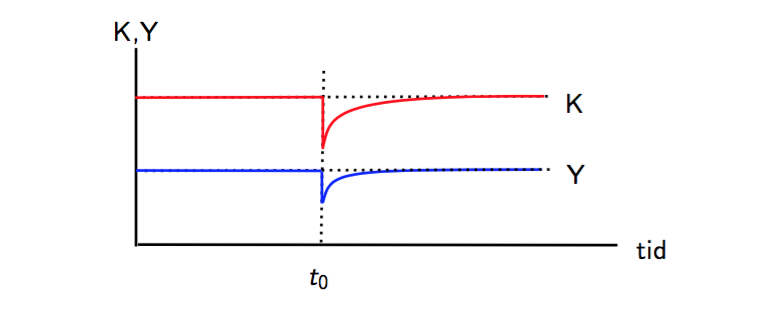
\includegraphics[scale=0.6]{skarm3}

\textbf{Befolkningsökning och teknisk utveckling} \par \noindent Den tillväxt som sker i befolkning och teknisk utveckling beskrivs med $ n = \frac{\Delta N}{N} \ g =  \frac{\Delta E}{E} $. BNP växer i takt med befolkning och teknsik utveckling. Detta på lång sikt. Med tillväxt så förväntar sig konsumenterna en högre inkomst imorgon, de spenderar mer idag, men alla kan inte låna mer i en sluten ekonomi. \par \noindent Konsumenterna måste "mutas" att inte spendera mer idag. \par

\textbf{Algoritm för att bestämma långsiktig BNP/capita: }
\begin{enumerate}
 \item Bestäm $ y = \frac{Y}{EN} $
 \item Sätt in med optimal kapitalstock, ta ut $ k^* $
 \item Sätt in den ekvationen som fås för $ k^* $ i orginal ekvationen för $ y = \frac{Y}{EN} $ som ger $ Y^* = (k^*)^{\alpha}EN $
\end{enumerate}


\vspace{5mm}
\title{Föreläsning 8}
\vspace{5mm} \par \noindent 





\bibliographystyle{plain}
\bibliography{references}

\end{document}
